% Supplementary Information. Numbers are filled by fill_numbers.py.
\documentclass[pdflatex,sn-mathphys-num]{sn-jnl}
\usepackage{graphicx}
\usepackage{amsmath,amssymb,amsfonts}
\usepackage{booktabs}
\newcommand{\Vbar}{\overline{\mathrm{Var}}}
\renewcommand{\thetable}{S\arabic{table}}
\renewcommand{\thefigure}{S\arabic{figure}}

%%BEGIN-NUMBERS
\newcommand{\Nrows}{20\,000}
\newcommand{\Nspecs}{20\,000}
\newcommand{\Nused}{19\,858}
\newcommand{\NallStruct}{142}
\newcommand{\Samples}{200}
\newcommand{\QubitLo}{2}
\newcommand{\QubitHi}{12}
\newcommand{\LayerLo}{1}
\newcommand{\LayerHi}{20}
\newcommand{\Narch}{5\,168}
\newcommand{\DesignSpace}{5\,280}
\newcommand{\MultMedian}{4}
\newcommand{\MultMax}{13}
\newcommand{\RowLeak}{95.0}
\newcommand{\BarrenFrac}{42.6}
\newcommand{\GlobalFrac}{50.4}
\newcommand{\LabelMean}{-1.88}
\newcommand{\LabelStd}{0.94}
\newcommand{\LabelMin}{-4.89}
\newcommand{\LabelMax}{-0.23}
\newcommand{\WithinVar}{0.010}
\newcommand{\TotalVar}{0.885}
\newcommand{\RsqCeiling}{0.989}
\newcommand{\RsqCeilingRy}{1.000}
\newcommand{\RsqCeilingPauli}{0.979}
\newcommand{\StructFracParams}{17.0}
\newcommand{\StructRowsAny}{87.0}
\newcommand{\LegacyFloorFrac}{9.6}
\newcommand{\LegacyCorr}{0.963}
\newcommand{\LegacyMAD}{0.16}
\newcommand{\LegacyFloorTrainable}{69}
\newcommand{\SpreadMedian}{0.6}
\newcommand{\SpreadPNineZero}{2.3}
\newcommand{\CostGap}{0.40}
\newcommand{\NFolds}{10}
\newcommand{\NFoldsK}{5}
\newcommand{\NRepeats}{2}
\newcommand{\RsqCV}{0.977}
\newcommand{\RsqCVsd}{0.003}
\newcommand{\MaeCV}{0.076}
\newcommand{\MaeCVsd}{0.004}
\newcommand{\AucCV}{0.998}
\newcommand{\AucCVsd}{0.000}
\newcommand{\AccCV}{0.980}
\newcommand{\AccCVsd}{0.003}
\newcommand{\RsqPhys}{0.682}
\newcommand{\RsqSub}{0.043}
\newcommand{\AucPhys}{0.927}
\newcommand{\GainOverPhys}{0.29}
\newcommand{\FracOfCeiling}{99}
\newcommand{\OofRsq}{0.978}
\newcommand{\OofRsqLo}{0.976}
\newcommand{\OofRsqHi}{0.979}
\newcommand{\RowRsq}{0.979}
\newcommand{\RowMae}{0.067}
\newcommand{\RowAuc}{0.999}
\newcommand{\ExtrapCut}{10}
\newcommand{\ExtrapTrainRows}{16\,278}
\newcommand{\ExtrapTestRows}{3\,580}
\newcommand{\RsqExtrap}{0.866}
\newcommand{\MaeExtrap}{0.313}
\newcommand{\RsqExtrapLo}{0.857}
\newcommand{\RsqExtrapHi}{0.874}
\newcommand{\MaeExtrapLo}{0.306}
\newcommand{\MaeExtrapHi}{0.320}
\newcommand{\RsqExtrapSeedSd}{0.002}
\newcommand{\AucExtrap}{0.991}
\newcommand{\RsqExtrapPhys}{0.326}
\newcommand{\MaeExtrapPhys}{0.665}
\newcommand{\RsqExtrapSub}{-1.027}
\newcommand{\RsqFull}{0.977}
\newcommand{\RsqPrim}{0.980}
\newcommand{\DeltaDerived}{-0.002}
\newcommand{\AblTopOne}{cost locality}
\newcommand{\AblTopOneDelta}{0.342}
\newcommand{\AblTopTwo}{entangler gate}
\newcommand{\AblTopTwoDelta}{0.183}
\newcommand{\AblTopThree}{entangle pattern}
\newcommand{\AblTopThreeDelta}{0.051}
\newcommand{\DeltaSize}{0.274}
\newcommand{\PythonVersion}{3.9.6}
\newcommand{\NumpyVersion}{2.0.2}
\newcommand{\SklearnVersion}{1.6.1}
\newcommand{\ValN}{200}
\newcommand{\ValState}{3.1e-16}
\newcommand{\ValGrad}{1.0e-15}
\newcommand{\ValGradN}{4\,792}
\newcommand{\ValStructN}{1153}
\newcommand{\ValStructViol}{0}
\newcommand{\RepeatN}{200}
\newcommand{\RepeatMAD}{0.021}
\newcommand{\RepeatMax}{0.20}
\newcommand{\MaeENOneOnelocal}{0.183}
\newcommand{\MaeEPNOneOnelocal}{0.805}
\newcommand{\RsqENOneOnelocal}{0.950}
\newcommand{\RsqEPNOneOnelocal}{0.220}
\newcommand{\RsqEMNOneOnelocal}{0.967}
\newcommand{\MaeEMNOneOnelocal}{0.132}
\newcommand{\MaeENOneOneglobal}{0.273}
\newcommand{\MaeEPNOneOneglobal}{0.438}
\newcommand{\RsqENOneOneglobal}{0.823}
\newcommand{\RsqEPNOneOneglobal}{0.199}
\newcommand{\RsqEMNOneOneglobal}{0.911}
\newcommand{\MaeEMNOneOneglobal}{0.119}
\newcommand{\MaeENOneTwolocal}{0.297}
\newcommand{\MaeEPNOneTwolocal}{0.907}
\newcommand{\RsqENOneTwolocal}{0.881}
\newcommand{\RsqEPNOneTwolocal}{0.163}
\newcommand{\RsqEMNOneTwolocal}{0.936}
\newcommand{\MaeEMNOneTwolocal}{0.209}
\newcommand{\MaeENOneTwoglobal}{0.488}
\newcommand{\MaeEPNOneTwoglobal}{0.516}
\newcommand{\RsqENOneTwoglobal}{0.624}
\newcommand{\RsqEPNOneTwoglobal}{0.188}
\newcommand{\RsqEMNOneTwoglobal}{0.927}
\newcommand{\MaeEMNOneTwoglobal}{0.152}
\newcommand{\MaeENOneOne}{0.230}
\newcommand{\MaeEPNOneOne}{0.615}
\newcommand{\RsqENOneOne}{0.923}
\newcommand{\RsqEPNOneOne}{0.347}
\newcommand{\RsqEMNOneOne}{0.957}
\newcommand{\MaeEMNOneOne}{0.125}
\newcommand{\MaeENOneTwo}{0.391}
\newcommand{\MaeEPNOneTwo}{0.713}
\newcommand{\RsqENOneTwo}{0.823}
\newcommand{\RsqEPNOneTwo}{0.307}
\newcommand{\RsqEMNOneTwo}{0.944}
\newcommand{\MaeEMNOneTwo}{0.181}
\newcommand{\MaeELocal}{0.243}
\newcommand{\MaeEPLocal}{0.859}
\newcommand{\RsqELocal}{0.911}
\newcommand{\RsqEPLocal}{0.189}
\newcommand{\RsqEMLocal}{0.950}
\newcommand{\MaeEMLocal}{0.172}
\newcommand{\MaeEGlobal}{0.381}
\newcommand{\MaeEPGlobal}{0.477}
\newcommand{\RsqEGlobal}{0.709}
\newcommand{\RsqEPGlobal}{0.202}
\newcommand{\RsqEMGlobal}{0.921}
\newcommand{\MaeEMGlobal}{0.136}
\newcommand{\RsqExtrapMLPLo}{0.944}
\newcommand{\RsqExtrapMLPHi}{0.955}
\newcommand{\AucCutmOnepFive}{0.996}
\newcommand{\BarrenCutmOnepFive}{60}
\newcommand{\AucCutmTwopZero}{0.998}
\newcommand{\BarrenCutmTwopZero}{43}
\newcommand{\AucCutmTwopFive}{0.999}
\newcommand{\BarrenCutmTwopFive}{27}
\newcommand{\AucCutmThreepZero}{0.998}
\newcommand{\BarrenCutmThreepZero}{15}
\newcommand{\RsqCVMLP}{0.978}
\newcommand{\AucCVMLP}{0.999}
\newcommand{\RsqExtrapMLP}{0.950}
\newcommand{\RsqCVRandomForest}{0.974}
\newcommand{\AucCVRandomForest}{0.997}
\newcommand{\RsqExtrapRandomForest}{0.862}
\newcommand{\RsqCVExtraTrees}{0.978}
\newcommand{\AucCVExtraTrees}{0.998}
\newcommand{\RsqExtrapExtraTrees}{0.865}
\newcommand{\RsqCVkNN}{0.967}
\newcommand{\AucCVkNN}{0.995}
\newcommand{\RsqExtrapkNN}{0.858}
\newcommand{\RsqCVLinearbaseline}{0.701}
\newcommand{\AucCVLinearbaseline}{0.952}
\newcommand{\RsqExtrapLinearbaseline}{0.338}
\newcommand{\ScreenSpearman}{0.988}
\newcommand{\ScreenTrainableFrac}{57.4}
\newcommand{\ScreenPrecFifty}{99.7}
\newcommand{\ScreenRecallFifty}{86.9}
\newcommand{\ScreenBottomTen}{100.0}
\newcommand{\ScreenTopPct}{20}
\newcommand{\ScreenTopK}{3\,971}
\newcommand{\GapHGBkSix}{-0.050}
\newcommand{\GapMLPkSix}{0.674}
\newcommand{\GapPhyskSix}{0.332}
\newcommand{\GapHGBkSeven}{0.288}
\newcommand{\GapMLPkSeven}{0.811}
\newcommand{\GapPhyskSeven}{0.330}
\newcommand{\GapHGBkEight}{0.548}
\newcommand{\GapMLPkEight}{0.881}
\newcommand{\GapPhyskEight}{0.324}
\newcommand{\GapHGBkNine}{0.730}
\newcommand{\GapMLPkNine}{0.915}
\newcommand{\GapPhyskNine}{0.324}
\newcommand{\GapHGBkTen}{0.866}
\newcommand{\GapMLPkTen}{0.950}
\newcommand{\GapPhyskTen}{0.326}
\newcommand{\LCHGBTwoFifty}{0.593}
\newcommand{\LCMLPTwoFifty}{0.752}
\newcommand{\LCHGBFiveHundred}{0.692}
\newcommand{\LCMLPFiveHundred}{0.866}
\newcommand{\LCHGBOneThousand}{0.819}
\newcommand{\LCMLPOneThousand}{0.919}
\newcommand{\LCHGBTwoThousand}{0.908}
\newcommand{\LCMLPTwoThousand}{0.950}
\newcommand{\LCHGBFourThousand}{0.959}
\newcommand{\LCMLPFourThousand}{0.968}
\newcommand{\LCHGBEightThousand}{0.972}
\newcommand{\LCMLPEightThousand}{0.975}
\newcommand{\LCHGBSixteenThousand}{0.978}
\newcommand{\LCMLPSixteenThousand}{0.978}
\newcommand{\LCRowsNinety}{2\,000}
\newcommand{\LCRowsSaturate}{4\,000}
\newcommand{\LopoExtraRows}{9\,926}
\newcommand{\LopoDescRsq}{0.974}
\newcommand{\LopoIndexRsq}{0.975}
\newcommand{\LopoLinearUnseen}{0.732}
\newcommand{\LopoLinearSeen}{0.980}
\newcommand{\LopoLinearPhys}{0.662}
\newcommand{\LopoLinearUnseenMae}{0.262}
\newcommand{\LopoLinearUnseenAuc}{0.964}
\newcommand{\LopoCircularUnseen}{0.694}
\newcommand{\LopoCircularSeen}{0.976}
\newcommand{\LopoCircularPhys}{0.685}
\newcommand{\LopoCircularUnseenMae}{0.298}
\newcommand{\LopoCircularUnseenAuc}{0.955}
\newcommand{\LopoAllUnseen}{0.414}
\newcommand{\LopoAllSeen}{0.970}
\newcommand{\LopoAllPhys}{0.507}
\newcommand{\LopoAllUnseenMae}{0.395}
\newcommand{\LopoAllUnseenAuc}{0.959}
\newcommand{\LopoBrickUnseen}{0.925}
\newcommand{\LopoBrickSeen}{0.977}
\newcommand{\LopoBrickPhys}{0.634}
\newcommand{\LopoBrickUnseenMae}{0.144}
\newcommand{\LopoBrickUnseenAuc}{0.983}
\newcommand{\LopoStarUnseen}{0.742}
\newcommand{\LopoStarSeen}{0.963}
\newcommand{\LopoStarPhys}{0.726}
\newcommand{\LopoStarUnseenMae}{0.286}
\newcommand{\LopoStarUnseenAuc}{0.980}
%%END-NUMBERS

\raggedbottom
\begin{document}
\title[Supplementary Information]{Supplementary Information for:
Predicting the Trainability of Hardware-Efficient Variational Quantum
Circuits: A Data-Driven Model for Barren Plateaus}
\author*[1]{\fnm{Md Habibur} \sur{Rahman}}\email{habib@gnu.ac.kr}
\affil*[1]{\orgdiv{Department of AI Convergence Engineering},
\orgname{Gyeongsang National University}, \orgaddress{\city{Jinju},
\country{Republic of Korea}}}
\abstract{This document collects tables and figures referenced from the main
text: model hyperparameters (Table~S1), descriptive statistics of the dataset
(Table~S2), sensitivity to the barren cutoff (Table~S3), the full model
comparison on the qubit-count extrapolation split (Table~S4), the
widening-gap extrapolation table (Table~S5), and the learning curve
(Figure~S1). Every number is produced by the released analysis scripts.}
\maketitle

\section{Model hyperparameters}
\begin{table}[t]
\centering
\caption{Model hyperparameters. Everything not listed is the scikit-learn
\SklearnVersion{} default. Features are standardized (zero mean, unit variance
on the training fold) for the linear, $k$-NN, and MLP models only.}
\label{tab:hyper}
\begin{tabular}{ll}
\toprule
\textbf{Model} & \textbf{Settings}\\
\midrule
Linear baseline & ridge, $\alpha=1$ / logistic regression, $C=1$\\
$k$-NN & $k=10$, uniform weights\\
MLP & hidden layers (128, 64), ReLU, Adam, 800 iterations\\
Random forest & 400 trees\\
Extra trees & 400 trees\\
HGB & 400 iterations, learning rate 0.08, 31 leaves\\
\botrule
\end{tabular}
\end{table}

\section{Descriptive statistics}
\begin{table}[t]
\centering
\caption{Descriptive statistics of the numeric features and the regression
label over the \Nused{} labeled circuits.}
\label{tab:datastats}
%%BEGIN-TABLE:datastats
\begin{tabular}{lrrrrrr}
\toprule
\textbf{Variable} & \textbf{Mean} & \textbf{Std} & \textbf{Min} & \textbf{25\%} & \textbf{Median} & \textbf{Max}\\
\midrule
\texttt{n\_qubits} & $7.02$ & $3.16$ & $2.00$ & $4.00$ & $7.00$ & $12.00$\\
\texttt{n\_layers} & $10.55$ & $5.77$ & $1.00$ & $6.00$ & $11.00$ & $20.00$\\
\texttt{n\_params} & $74.02$ & $55.48$ & $2.00$ & $28.00$ & $60.00$ & $240.00$\\
\texttt{n\_entanglers} & $136.63$ & $198.79$ & $1.00$ & $28.00$ & $70.00$ & $1320.00$\\
\texttt{depth\_ratio} & $2.01$ & $1.83$ & $0.08$ & $0.80$ & $1.50$ & $10.00$\\
structural-zero fraction & $0.22$ & $0.25$ & $0.00$ & $0.05$ & $0.12$ & $0.99$\\
$\log_{10}\overline{\mathrm{Var}}$ (label) & $-1.88$ & $0.94$ & $-4.89$ & $-2.62$ & $-1.78$ & $-0.23$\\
\botrule
\end{tabular}
%%END-TABLE:datastats
\end{table}

\section{Sensitivity to the barren cutoff}
Main-text Section~4.4 discusses this table.
\begin{table}[t]
\centering
\caption{Classification with alternative barren cutoffs $y<c$. AUC is the
mean $\pm$ standard deviation over \NFoldsK{} architecture-grouped folds.}
\label{tab:cutoff}
%%BEGIN-TABLE:cutoff
\begin{tabular}{lcc}
\toprule
Cutoff $y<c$ & Barren fraction & AUC (grouped CV) \\
\midrule
$c=-1.5$ & 59.7\% & $0.996 \pm 0.001$ \\
$c=-2.0$ & 42.6\% & $0.998 \pm 0.000$ \\
$c=-2.5$ & 27.0\% & $0.999 \pm 0.000$ \\
$c=-3.0$ & 15.0\% & $0.998 \pm 0.001$ \\
\botrule
\end{tabular}
%%END-TABLE:cutoff
\end{table}

\section{Qubit-count extrapolation: all learners}
Main-text Section~4.2 discusses this table; the per-subset breakdown with
confidence intervals is main-text Table~8.
\begin{table}[t]
\centering
\caption{Extrapolation split: trained on $n\le\ExtrapCut$
(\ExtrapTrainRows{} circuits), tested on $n\in\{11,12\}$ (\ExtrapTestRows{}
circuits). Single split; see Table~\ref{tab:extrapbreak} for confidence
intervals.}
\label{tab:extrap}
%%BEGIN-TABLE:extrap
\begin{tabular}{lcccc}
\toprule
Model & $R^2$ & MAE & AUC & Accuracy \\
\midrule
\textbf{Hist Gradient Boosting} & 0.866 & 0.313 & 0.991 & 0.972 \\
MLP & 0.950 & 0.154 & 0.997 & 0.977 \\
Random Forest & 0.862 & 0.310 & 0.996 & 0.977 \\
Extra Trees & 0.865 & 0.306 & 0.993 & 0.976 \\
k-NN & 0.858 & 0.321 & 0.979 & 0.968 \\
Linear baseline & 0.338 & 0.680 & 0.842 & 0.810 \\
\midrule
Physics-informed linear & 0.326 & 0.665 & 0.814 & 0.752 \\
Cost-locality subgroup mean & -1.027 & 1.326 & 0.699 & 0.248 \\
Training mean & -1.125 & 1.359 & 0.500 & 0.248 \\
\botrule
\end{tabular}
%%END-TABLE:extrap
\end{table}

\section{Extrapolation with a widening gap}
Main-text Section~4.2 and Figure~5 discuss this table.
\begin{table}[t]
\centering
\caption{Extrapolation with a widening gap: train on $n\le k$, test on all
$n>k$.}
\label{tab:gap}
%%BEGIN-TABLE:gap
\begin{tabular}{crrcccccc}
\toprule
 & & & \multicolumn{2}{c}{HGB} & \multicolumn{2}{c}{MLP} & \multicolumn{2}{c}{Physics-linear} \\
\cmidrule(lr){4-5}\cmidrule(lr){6-7}\cmidrule(lr){8-9}
Train $n\le k$ & Train rows & Test rows & $R^2$ & MAE & $R^2$ & MAE & $R^2$ & MAE \\
\midrule
$k=6$ & 8916 & 10942 & -0.050 & 0.732 & 0.674 & 0.344 & 0.332 & 0.519 \\
$k=7$ & 10671 & 9187 & 0.288 & 0.615 & 0.811 & 0.285 & 0.330 & 0.552 \\
$k=8$ & 12572 & 7286 & 0.548 & 0.514 & 0.881 & 0.224 & 0.324 & 0.591 \\
$k=9$ & 14448 & 5410 & 0.730 & 0.421 & 0.915 & 0.195 & 0.324 & 0.630 \\
$k=10$ & 16278 & 3580 & 0.866 & 0.313 & 0.950 & 0.154 & 0.326 & 0.665 \\
\botrule
\end{tabular}
%%END-TABLE:gap
\end{table}

\section{Learning curve}
Main-text Section~4.7 discusses this figure.
\begin{figure}[t]
\centering
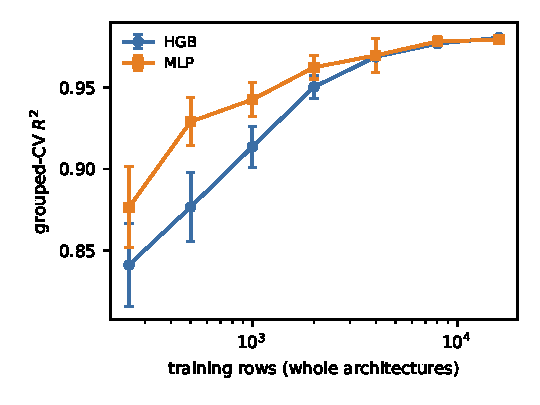
\includegraphics[width=0.6\textwidth]{figs/learning_curve.pdf}
\caption{Learning curve: architecture-grouped CV $R^2$ against the number
of training rows. Error bars: standard deviation over the five folds.}
\label{fig:learningcurve}
\end{figure}

\end{document}
